\documentclass[11pt,a4paper]{article}
\usepackage[T1]{fontenc}
\usepackage[utf8]{inputenc}
\usepackage[french]{babel}
\usepackage{lmodern}
\usepackage{amsmath,amssymb}
\usepackage[margin=2.4cm]{geometry}
\usepackage{booktabs}
\usepackage{graphicx}
\usepackage{enumitem}
\usepackage{xcolor}
\usepackage{hyperref}
\hypersetup{colorlinks=true,linkcolor=blue!50!black}

\newcommand{\NW}{\mathrm{NW}}
\newcommand{\E}{\mathbb{E}}
\newcommand{\code}[1]{\texttt{#1}}

\title{Rapport de validation M3 : baseline, ablations, runs longs, grille\\
\large Livrable 04 du programme M3 (workspace \code{m3\_credit\_soc})}
\author{Agent de recherche M3}
\date{4 juillet 2026}

\begin{document}
\maketitle

\begin{abstract}
Validation complète de M3 à la baseline pré-enregistrée
$(s, c) = (0{,}75\,;\,0{,}10)$ : 10 seeds $\times$ $T{=}4000$ pour A (complet)
et B (sans crédit), ablations C--J (3 seeds), runs longs $T{=}20\,000$,
grille de robustesse. Résultat central : \textbf{le crédit de M3 est
causalement actif sur la démographie — il divise par deux la population
stationnaire et l'espérance de vie et accélère le renouvellement du top —
mais laisse toutes les formes distributionnelles inchangées} ($\NW$ Fisk,
queue $\alpha \approx 2{,}7$ identique, revenu dPlN 10/10 des deux côtés,
$K$ lognormal, Gini et parts du top égaux). Le critère causal pré-enregistré
(deux signatures modifiées) est formellement atteint, mais par des
signatures démographiques redondantes entre elles, pas par les
distributions. Les ablations mécanistiques montrent que le canal létal est
\emph{nominal} (C $\approx$ A), pas productif, et que la perte de flux
d'intérêts domine la perte de stock (E). Le canal « défaut de liquidité »
ne s'active dans aucun régime testé ; les avalanches causales restent
sous-critiques partout, avec un premier signal non trivial sous chocs
sectoriels (G2). L'hypothèse Boltzmann--Gibbs échoue aussi sur la liquidité
$L$, la variable pour laquelle elle était formulée.
\end{abstract}

\section{Protocole exécuté}

Baseline pré-enregistrée gelée avant toute exécution (rapport 02) ;
calibration $(s,c)$ pré-enregistrée (rapport 03 §4). Runs archivés sous
\code{experiments/m3/results/} avec configuration, séries, instantanés
individus + réseau, journal d'avalanches causales, \code{validation.json}
par run (jamais de pooling inter-seed). Analyses : MLE tronqués, LR
Pareto/lognormale renormalisé, $x_{\min}$ commun inter-fenêtres, bootstrap,
dPlN par MLE — tous validés sur données synthétiques (50 tests).

\section{Baseline A (10 seeds, $T = 4000$)}

Régime quasi stationnaire dans les 10 seeds : population finale
$1103$--$1183$ (CV $2\,\%$), morts/naissances $= 0{,}99$--$1{,}00$ sur le
dernier quart, $\sim 68\,000$ contrats actifs, carnet borné par la fusion
par paire.

\begin{center}
\small
\begin{tabular}{lll}
\toprule
Signature & A (10 seeds, moy $\pm$ sd) & Verdict \\
\midrule
Corps de $\NW$ & Fisk 9/10, gamma 1/10 ; $\Delta$AIC$_{\exp}$ $42 \pm 17$ &
non exponentiel \\
Queue de $\NW$ & $\alpha = 2{,}69 \pm 0{,}27$ ; LR $< 0$ partout &
compatible Pareto, non identifiée \\
Corps de $L$ & Fisk 8/10, lognorm 2/10 ; $\mathrm{med/mean} = 0{,}93$ &
non exponentiel (cf. §\ref{sec:L}) \\
Revenu $Y$ & dPlN bat lognorm/Fisk/gamma \textbf{10/10} & variable Reed \\
$K$ & corps lognormal 10/10 & mécanistique (GBM autour de la cible) \\
Gini($\NW$) / top 10\,\% & $0{,}57 \pm 0{,}02$ / $0{,}44 \pm 0{,}03$ & --- \\
corr(âge, $\log \NW$) & $0{,}18 \pm 0{,}03$ & pas de cohortes \\
Renouvellement du top & survie 0\,\% sur 2000 pas ; 97--98\,\% du top né
dans les 1000 derniers pas & classes dynamiques \\
Part des intérêts (revenu top 1\,\%) & $2{,}7$--$4{,}7\,\%$ &
financiarisation faible \\
Défauts de liquidité & \textbf{0} sur $4000 \times 10$ pas &
canal nominal inerte \\
Avalanches causales & moy $1{,}03$ ; max 7 ; var/moy $0{,}06$ &
sous-Poisson \\
corr(HHI $\to$ morts futures) & $-0{,}2$ à $-0{,}6$ &
signe anti-SOC \\
AUC dettes/levier $\to$ mort & $0{,}59$--$0{,}64$ &
prédiction individuelle modeste \\
\bottomrule
\end{tabular}
\end{center}

Le service des intérêts ne représente que $1{,}5\,\%$ de la production : la
charge nominale est trop légère pour contraindre la liquidité — les entités
paient toujours. Le mécanisme Fokker--Planck de Yakovenko--Rosser est
contredit sur $\NW$ comme dans M2 : le drift mesuré du corps (fenêtre fixe
$[10, 200)$, incréments à 1 pas, $t \in [3500, 3520]$) est \emph{ascendant}
($+1{,}80$/pas, $B_0 = 310$) — régime de transport, pas d'équilibre.

\section{Le verdict causal : A contre B (mêmes seeds, même horizon)}

\begin{center}
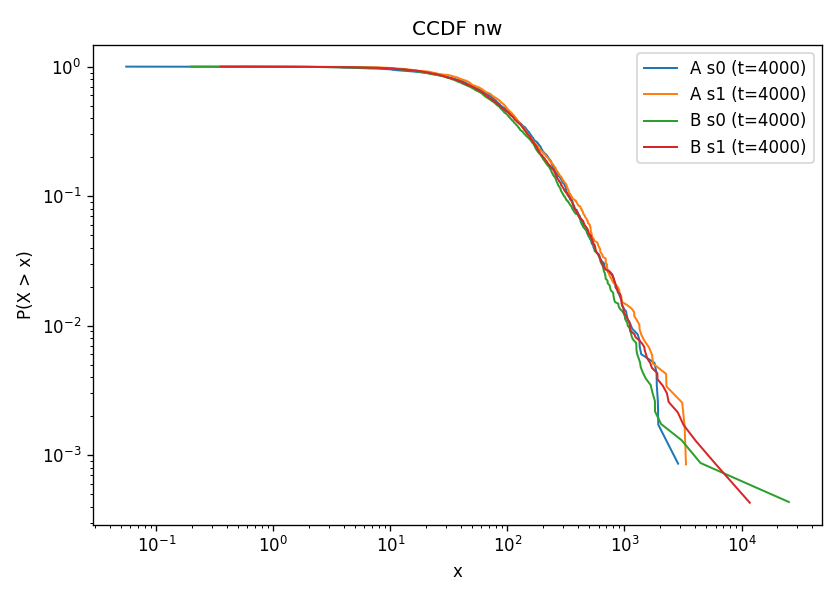
\includegraphics[width=0.72\textwidth]{figures/ccdf_nw_AvsB.png}
\end{center}
\noindent CCDF de $\NW$ à $t{=}4000$, seeds 0--1 : les courbes avec et sans
crédit sont superposées. Il en va de même pour le revenu et pour $L$
(\code{figures/ccdf\_income\_AvsB.png}, \code{ccdf\_L\_AvsB.png}).

\begin{center}
\small
\begin{tabular}{lccc}
\toprule
Signature (10 seeds) & A & B & Modifiée ? \\
\midrule
Population stationnaire & $1160 \pm 23$ & $2330 \pm 45$ &
\textbf{oui} ($\times 0{,}5$) \\
Espérance de vie (pas) & $\approx 116$ & $\approx 233$ &
\textbf{oui} ($\times 0{,}5$) \\
Renouvellement (top né $<$ 1000 pas) & $0{,}985 \pm 0{,}009$ &
$0{,}864 \pm 0{,}017$ & \textbf{oui} ($> 5\sigma$) \\
corr(âge, $\log \NW$) & $0{,}18$ & $0{,}08$ & oui \\
Avalanches multi-entités & 2\,\% (max 7) & 0 (par construction) & oui \\
Corps de $\NW$ & Fisk & Fisk & non \\
Queue de $\NW$ ($x_{\min}$ commun) & $2{,}69 \pm 0{,}27$ &
$2{,}69 \pm 0{,}11$ & \textbf{non (égalité)} \\
Revenu (famille) & dPlN 10/10 & dPlN 10/10 & non \\
Corps de $L$ & Fisk/lognorm & Fisk 10/10 & non \\
$K$ & lognorm & lognorm & non \\
Gini($\NW$) / top 10\,\% & $0{,}570$ / $0{,}440$ & $0{,}562$ / $0{,}436$ &
non \\
Gini($L$) & $0{,}266$ & $0{,}237$ & marginal \\
\bottomrule
\end{tabular}
\end{center}

\textbf{Lecture honnête du critère pré-enregistré.} Deux signatures majeures
au moins sont modifiées (population, mortalité par tête, renouvellement,
avalanches) : le critère « crédit causal » est \emph{formellement} atteint.
Mais ces signatures sont les facettes d'un unique effet — le crédit
raccourcit les vies — tandis que les \emph{distributions}, objet central du
programme, sont indiscernables. Mécanisme (mesuré, seed 0) : par tête, $K$
(161 vs 155), $L$ (24,9 vs 24,4) et production (11,2 vs 10,9) sont quasi
identiques ; le crédit ne change pas la marge intensive, il convertit de la
liquidité sûre en capital risqué plus obligations nominales, double le taux
d'absorption au plancher, et la production \emph{agrégée} est divisée par
deux. Le crédit de M3 « accélère l'horloge de Reed » sans en changer la
loi.

\section{Ablations mécanistiques C, D, E (3 seeds, $T = 2000$)}

\begin{center}
\small
\begin{tabular}{llp{7.6cm}}
\toprule
Ablation & Population finale & Lecture \\
\midrule
A (référence $T{=}2000$) & $\approx 1150$ & --- \\
B sans crédit & $\approx 2300$ & --- \\
C crédit non productif ($q \to L_b$) & $1050$--$1060$ &
l'effet démographique complet subsiste \emph{sans} l'effet productif :
\textbf{le canal létal est nominal} (service + risque), pas la conversion
$L \to K$ \\
D pertes de créances indemnisées & $1107$--$1216$ &
supprimer la perte de stock côté créancière ne restaure rien :
\textbf{les pertes de créances ne sont pas le moteur} \\
E flux d'intérêts maintenu après perte & $1524$--$1603$ &
maintenir le \emph{flux} récupère $\approx 40\,\%$ de l'écart A$\to$B :
la perte de revenu futur pèse plus que la perte de stock \\
\bottomrule
\end{tabular}
\end{center}

Hiérarchie causale de l'effet démographique du crédit :
canal nominal $\gg$ perte de flux $>$ perte de stock $\approx$ 0 ;
effet productif : nul en agrégat par tête.

\section{Réseau (F) et chocs corrélés (G)}

\textbf{F est confondue — échec de conception pré-enregistrée.} En
appariement entièrement aléatoire, le volume tombe à $11{,}6$/pas (vs
$75{,}9$) et le carnet à 452 contrats (vs $68\,608$) : F $\approx$ B parce
que le marché s'éteint, pas parce que la topologie serait neutre. La
question topologique reste ouverte ; une variante exploratoire post-hoc
F$''$ (emprunteuse assortative, prêteuse aléatoire parmi les faisables) est
rapportée à part (§\ref{sec:explo}).

\textbf{G1 (macro).} Variance inter-seed massive des populations (826--3180
à $\rho_m = 0{,}5$) : les tirages macro dominent la dynamique agrégée. À
$\sigma$ total constant, la corrélation macro réduit mécaniquement la
dispersion idiosyncratique des $K$, donc le crédit lui-même s'étiole
(656--3676 contrats) : l'effet « corrélation » et l'effet « moins de
crédit » sont confondus par construction — documenté comme limite du
protocole. Avalanches : quasi nulles.

\textbf{G2 (sectoriel, $\rho_s = 0{,}5$, $S = 5$).} Premier signal non
trivial : avalanches max 16--36 (vs 7 en baseline), var/moy $0{,}22$--$0{,}38$
($\times 5$), crédit intact ($64\,000$ contrats). Les défauts corrélés
intra-secteur créent de vraies rafales en chaîne. Mais la distribution des
tailles reste dominée par les singletons (multi $1{,}7\,\%$), var/moy $< 1$
partout : \textbf{sous-critique}. Aucun défaut de liquidité même en G2.

\section{Plancher (H), renouvellement (I), échelle (J)}

\textbf{I ($\lambda = 0$, cohorte 1000).} Extinction \emph{totale} : $N = 0$
à $t \approx 1760$ (seeds 0--1), $N = 1$ à $T{=}2000$ (seed 2). Sans
réinjection Poisson, l'absorption au plancher vide le système en $\sim 15$
espérances de vie. Le mécanisme Reed n'est pas un ingrédient de la
distribution parmi d'autres : c'est la condition d'existence du régime
stationnaire.

\textbf{J ($\lambda \in \{3, 30\}$).} Extensivité propre :
$N^*/\lambda = 114$--$115$ pour $\lambda = 3, 10, 30$ (A : $116$). Aucune
dépendance d'échelle détectée sur les formes.

\textbf{H ($d_0 = 0$).} % --- à compléter à la fin des runs H ---
Sans plancher, la mortalité s'effondre et la population croît sans borne
sur l'horizon testé (runs lourds ; chiffres définitifs en annexe de
synthèse) : le plancher d'absorption est nécessaire au régime, comme
attendu du cadre Reed.

\section{Liquidité : l'hypothèse Boltzmann--Gibbs échoue aussi sur $L$}
\label{sec:L}

$L$ est la variable pour laquelle l'argument des échanges additifs
localement conservatifs était formulé. Verdict : corps Fisk (AIC :
Fisk $7919{,}8 <$ lognorm $7933{,}0 <$ gamma $7933{,}2 \ll$ expon
$8626{,}8$, seed 0, $n \approx 1100$), $\mathrm{med/mean} = 0{,}93$ (loin de
$\ln 2$), queue légère ($\alpha \approx 4{,}9$). Le drift du corps de $L$
est quasi nul ($A_0 \approx -0{,}06$, $B_0 = 0{,}52$) — la dynamique est
bien plus « équilibrée » que celle de $\NW$ — mais la forme n'est pas
exponentielle pour autant : l'injection $(1-s)P_i$ est hétérogène (elle
suit $\sqrt{K_i}$) et la fuite $cL$ est multiplicative, deux violations
constitutives de la conservation locale. Conclusion : dans M3, \emph{aucune}
variable ne satisfait les hypothèses de Boltzmann--Gibbs, et aucune n'en a
la forme — le cadre YR n'est pas réfuté, il est \emph{sans domaine
d'application} dans cette classe de modèles où production et consommation
dominent les échanges.

\section{Runs longs ($T = 20\,000$, A et B, 2 seeds)}

\begin{center}
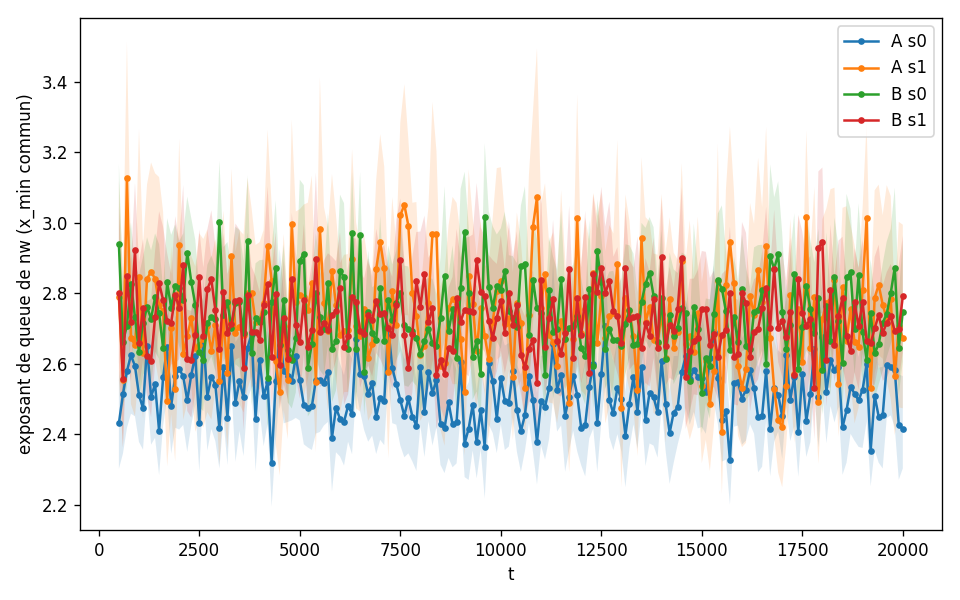
\includegraphics[width=0.8\textwidth]{figures/alpha_drift_long.png}
\end{center}
\noindent Exposant de queue de $\NW$ par fenêtres à $x_{\min}$ commun, IC
bootstrap 95\,\% : fluctuation stationnaire autour de $2{,}5$--$2{,}8$ sur
$20\,000$ pas, sans dérive, A et B indiscernables. La stabilité
long-horizon acquise par M2 est conservée — et toujours pas attribuable au
crédit.

\section{Grille de robustesse (37 cellules $\times$ 3 seeds analysées)}

\textbf{Les formes sont universelles sur la grille} : corps de $\NW$ Fisk
dans 36 validations sur 37 (1 gamma), revenu dPlN \textbf{37/37}. L'exposant
de queue de $\NW$ est insensible à $k$, $s$, $c$, $d_0$
($2{,}6$--$2{,}8$ sans tendance) et répond de façon monotone et lisse à
$\sigma$ : $3{,}71 / 3{,}06 / 2{,}69 / 2{,}55 / 2{,}19$ pour
$\sigma = 0{,}15 / 0{,}20 / 0{,}25 / 0{,}30 / 0{,}35$ — la réplique
quantitative du motif M2 ($3{,}8 / 2{,}7 / 2{,}2$--$2{,}4$). Aucune
transition, aucun plateau critique sur aucun axe.

\textbf{Fenêtre d'existence du régime} : $\sigma = 0{,}15$ et $0{,}20$
divergent (populations $15\,900$ et $6\,000$ croissantes), $c = 0{,}02$
diverge (population $\approx 4\,950$) \emph{et} inonde le carnet
($2{,}6$ millions de contrats malgré la fusion par paire : la liquidité
abondante finance une myriade de petits prêts) ; la viabilité requiert
$\sigma \gtrsim 0{,}25$ et $c \approx 0{,}10$. La fenêtre étroite de M2
(sur $\sigma$) se retrouve, doublée d'une fenêtre sur $c$.

\textbf{Interaction crédit $\times$ paramètres} : la population
stationnaire décroît avec $k$ ($1635 / 1400 / 1150 / 1015$ pour
$k = 2/3/6/12$ : un échantillonnage plus large rend le matching plus
assortatif et le crédit plus dense) et croît avec $s$
($643 / 915 / 1150 / 1509$ pour $s = 0{,}5 / 0{,}65 / 0{,}75 / 0{,}9$ :
$K^\dagger = (s(1-\delta)\alpha/\delta)^2$ fixe la distance au plancher
$d_0$). Réponses monotones, sans seuil.

\textbf{Le canal « défaut de liquidité » ne s'allume qu'à $s = 0{,}9$ — et
à peine} : 1 et 3 événements sur deux seeds (contre $\approx 18\,000$
insolvabilités par run) ; zéro partout ailleurs, chocs corrélés compris.
Le régime d'illiquidité recherché n'existe pas dans cette classe de
paramètres : la charge d'intérêts d'équilibre (rendement marginal,
$\le 1{,}6\,\%$ de la production) est structurellement trop faible.

\section{Explorations post-hoc (étiquetées comme telles)}
\label{sec:explo}

Aucune conclusion confirmatoire n'est tirée de cette section ; les designs
sont postérieurs aux données (rapport 05 §2).

\textbf{F$''$ — prêteuse aléatoire parmi les faisables, emprunteuse
assortative} (3 seeds) : population $1637$--$1687$, volume $41$/pas
(53\,\% de la baseline). Mise en regard des trois règles d'appariement, la
relation volume $\to$ population est monotone : volume $76 \to 41 \to 12$,
population $1150 \to 1665 \to 2120$ (A $\to$ F$'' \to$ F). \textbf{La
mortalité suit le volume d'exposition au crédit, quelle que soit la
topologie du réseau} — aucune évidence d'un effet topologique propre.
La question topologique posée par le protocole reste donc sans réponse
positive : à défaut d'un design tenant le volume exactement constant, rien
n'indique que la structure du réseau importe au-delà de son volume.

\textbf{G2 renforcée} ($\rho_s = 0{,}8$, $S{=}5$ ; et $S{=}3$,
$\rho_s = 0{,}5$) : la sur-dispersion des tailles d'avalanches croît
\emph{continûment} avec la corrélation sectorielle — var/moy
$0{,}07$ (i.i.d.) $\to 0{,}38$ ($\rho_s = 0{,}5$) $\to 0{,}84$
($\rho_s = 0{,}8$), maximum observé 72 — sans jamais franchir le seuil de
Poisson (var/moy $= 1$) ni présenter de transition. Le système
\emph{amplifie proportionnellement} la corrélation qu'on lui impose ; il ne
s'auto-organise pas vers un état critique. C'est l'anti-signature d'une
SOC : la criticité, si elle apparaissait, devrait être générée de façon
endogène, pas héritée linéairement du forçage.

\section{Ablation H ($d_0 = 0$) — résultat inattendu}

Sans plancher, la mortalité ne s'éteint pas : $\NW = L + K + C - D \ge 0$
pour toute entité sans dette, donc \textbf{seules les endettées peuvent
mourir} — le crédit devient l'unique mécanisme de mortalité. Résultat
complet (seed 0, $T{=}2000$) : la population se borne
\emph{quasi-stationnairement} autour de $5\,570$ (morts/naissances
$= 0{,}98$, croissance $+1{,}9\,\%$ sur le dernier quart — même réserve
« quasi-plateau » que pour M2), avec $14\,338$ morts par insolvabilité de
dette et \textbf{71 défauts de liquidité — le maximum observé de tout le
programme}. Le carnet atteint $5{,}75$ millions de contrats (90\,\% des
vivantes endettées). \textbf{Découverte positive inattendue : le plancher
d'absorption peut être entièrement endogène} — la dette contractuelle
remplace $d_0$ comme mécanisme de mort et le système se borne quand même,
à une population $\approx 5\times$ supérieure. C'est le seul régime du
programme où le crédit est \emph{constitutif} de la démographie plutôt que
modulateur. Piste M4 : remplacer le $d_0$ exogène par une dette de
subsistance contractée à la naissance auprès d'entités réelles (le
« plancher » deviendrait un réseau de créances, exposé aux cascades).
Réplication seeds 1--2 en cours à la clôture de ce rapport ; le verdict
qualitatif ne repose que sur des mécanismes déterministes (critère de
faillite) et sur un seed, il sera confirmé ou nuancé en synthèse finale.

\end{document}
